\documentclass[t]{beamer}
\mode<presentation>

\usepackage{etex}

\usetheme{Madrid}
% other themes: Warsaw, AnnArbor, Antibes, Bergen, Berkeley, Berlin, Boadilla, boxes, CambridgeUS, Copenhagen, Darmstadt, default, Dresden, Frankfurt, Goettingen,
% Hannover, Ilmenau, JuanLesPins, Luebeck, Madrid, Maloe, Marburg, Montpellier, PaloAlto, Pittsburg, Rochester, Singapore, Szeged, classic

\setbeamertemplate{navigation symbols}{\insertslidenavigationsymbol}

\usecolortheme{dolphin}
%\usecolortheme{seagull}
% color themes: albatross, beaver, beetle, crane, default, dolphin, dov, fly, lily, orchid, rose, seagull, seahorse, sidebartab, structure, whale, wolverine

%\usefonttheme{serif}
% font themes: default, professionalfonts, serif, structurebold, structureitalicserif, structuresmallcapsserif

% pdf is displayed in full screen mode automatically
%\hypersetup{pdfpagemode=FullScreen}

%\AtBeginSection[]
%{
%  \begin{frame}<beamer>
%    \frametitle{Outline}
%    \tableofcontents[currentsection,currentsubsection]
%  \end{frame}
%}

% define your own colours:
\definecolor{Red}{rgb}{1,0,0}
\definecolor{Blue}{rgb}{0,0,1}
\definecolor{Green}{rgb}{0,1,0}
\definecolor{magenta}{rgb}{1,0,.6}
\definecolor{lightblue}{rgb}{0,.8,1}
\definecolor{lightpurple}{rgb}{.6,.4,1}
\definecolor{gold}{rgb}{.6,.5,0}
\definecolor{orange}{rgb}{1,0.4,0}
\definecolor{hotpink}{rgb}{1,0,0.5}
\definecolor{newcolor2}{rgb}{.5,.3,.5}
\definecolor{newcolor}{rgb}{0,.3,1}
\definecolor{newcolor3}{rgb}{1,0,.35}
\definecolor{darkgreen1}{rgb}{0, .35, 0}
\definecolor{darkgreen}{rgb}{0, .6, 0}
\definecolor{darkred}{rgb}{.75,0,0}

\xdefinecolor{olive}{cmyk}{0.64,0,0.95,0.4}
\xdefinecolor{purpleish}{cmyk}{0.75,0.75,0,0}

%\usepackage{beamerinnerthemerounded}
% inner themes include circles, default, inmargin, rectangles, rounded

%\usepackage{beamerouterthemesmoothbars}
% outer themes include default, infolines, miniframes, shadow, sidebar, smoothbars, smoothtree, split, tree

\useoutertheme[subsection=false]{smoothbars}

% to have the same footer on all slides
\setbeamertemplate{footline}[text line]{
\raisebox{3pt}{
\includegraphics[height=15pt]{su-long.eps}}\hfill 
\raisebox{5pt}{Math 207:  Statistics}\hfill 
\raisebox{5pt}{Sample Surveys}\hfill
\raisebox{5pt}{\insertframenumber/\pageref{lastpage}}}
%\setbeamertemplate{footline}[text line]{} % or empty footer

% include packages
\usepackage{subfigure}
\usepackage{multicol}
\usepackage{amsmath}
\usepackage{epsfig}
\usepackage{graphicx}
\usepackage[all,knot]{xy}
\xyoption{arc}
\usepackage{url}
\usepackage{multimedia}
\usepackage{hyperref}
\usepackage{setspace}

\title{Math 207:  Statistics}
\subtitle{Chapter 19:  Samplel Surveys}
\author{Ralph Wojtowicz}
\institute{Mathematics Department\\ Shenandoah University}
%\date{\scriptsize 17 February 2012}

\usepackage{pstricks,pst-grad,pst-func,pst-text,pst-node,multido,pst-plot,calc,pst-3dplot}

\newcommand{\BRACE}{
\begin{pspicture}(-3,-2.1)(3,1.1)
\psset{yunit=3,linewidth=0.02}
\psline(-3.5,0)(3.5,0)  
  \psline(-3,0)(-3,-0.04) \rput[t](-3,-0.07){\scriptsize -3\hphantom{-}}
  \psline(-2,0)(-2,-0.04) \rput[t](-2,-0.07){\scriptsize -2\hphantom{-}}
  \psline(-1,0)(-1,-0.04) \rput[t](-1,-0.07){\scriptsize -1\hphantom{-}}
  \psline(0,0)(0,-0.04)   \rput[t](0,-0.07){\scriptsize 0}
  \psline(1,0)(1,-0.04)   \rput[t](1,-0.07){\scriptsize 1}
  \psline(2,0)(2,-0.04)   \rput[t](2,-0.07){\scriptsize 2}
  \psline(3,0)(3,-0.04)   \rput[t](3,-0.07){\scriptsize 3}
  \rput[l](3.6,0){\scriptsize $x$}
\psline(0,0)(0,0.5)
  \psline(-0.12,0.5)(0,0.5)    \rput[r](-0.21,0.5){\scriptsize $0.5$}
  \psline(-0.12,0.25)(0,0.25)  \rput[r](-0.21,0.25){\scriptsize $0.25$}
\psGauss[linecolor=blue,linewidth=0.02,sigma=1,mue=0]{-3}{3}
\pnode(-1,-0.15){A}\pnode(1,-0.15){B}
\psbrace[braceWidth=0.02,braceWidthInner=5pt,braceWidthOuter=5pt](A)(B){\rput{90}(0.25,-0.05){\scriptsize 68\%}}
%
\pnode(-2,-0.15){C}\pnode(2,-0.15){D}
\psbrace[braceWidth=0.02,braceWidthInner=25pt,braceWidthOuter=5pt](C)(D){\rput{90}(0.25,-0.05){\scriptsize 95\%}}
%
\pnode(-3,-0.15){E}\pnode(3,-0.15){F}
\psbrace[braceWidth=0.02,braceWidthInner=45pt,braceWidthOuter=5pt](E)(F){\rput{90}(0.25,-0.1){\scriptsize 99.7\%}}
\end{pspicture}}

\begin{document}

%\frame[plain]{
%	\titlepage
%}


\begin{frame}[plain]
\definecolor{myblue}{rgb}{0,0,0.6}
\definecolor{grayA}{rgb}{0.95,0.95,0.95}
\definecolor{grayB}{rgb}{0.98,0.98,0.98}
\begin{center}

%\begin{pspicture}(0,0)(7,4.8)
\begin{pspicture}(-6,-7)(6,2)

%\rput(0,-1.85){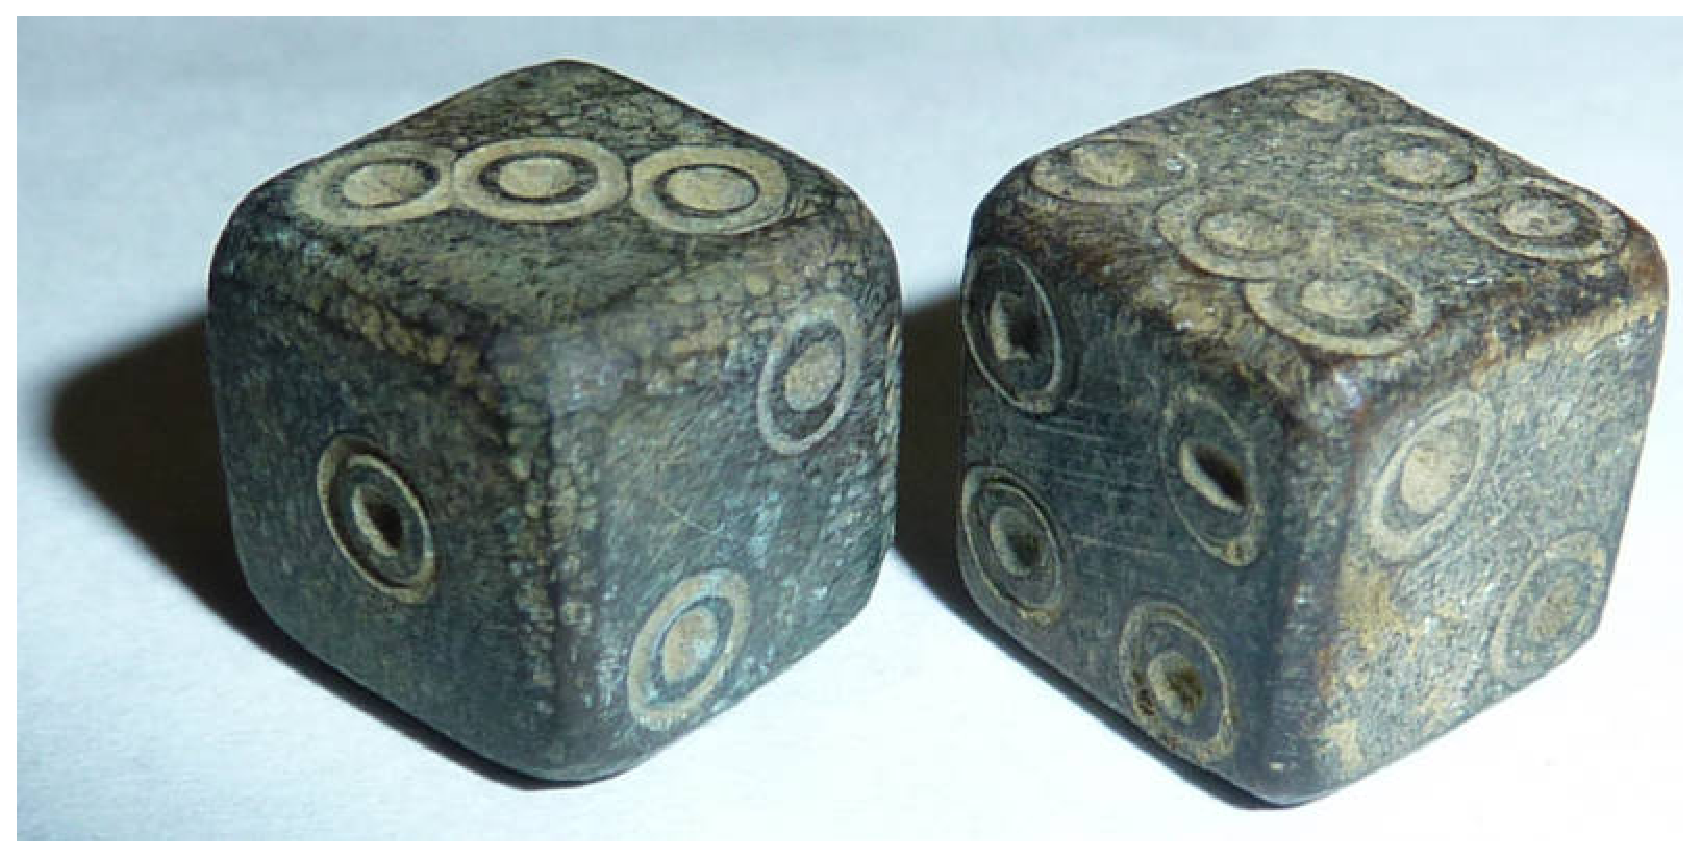
\includegraphics[height=4.2cm]{dice.eps}}
\psframe[linewidth=0.02,linecolor=gray](-6.2,-7)(6.2,2.2)
\psframe[linewidth=0.02,linecolor=gray](-6.15,-6.95)(6.15,2.15)
\rput(0,1.4){\color{myblue}\large Math 207:  Statistics}
\rput(0,0.6){\color{myblue}Chapter 19:  Sample Surveys}
%
\psframe[linewidth=0.02,fillstyle=solid,fillcolor=grayA](-2,-3)(2,-1)
  \rput[tl](-1.9,-1.1){\tiny Population (parameters)}
\psframe[linewidth=0.02,fillstyle=solid,fillcolor=grayB](-0.25,-2.75)(1.75,-2)
  \rput[tl](-0.15,-2.1){\tiny Sample (statistics)}
%\psframebox(0,0)(4,4)
\rput(0,-4.5){\scriptsize Dr.~Ralph Wojtowicz}
\rput(0,-5.0){\scriptsize Mathematics Department}
\rput(0,-5.8){
\includegraphics[height=1cm]{su-long.eps}}
%
%\rput(0,-6.5){\scriptsize 17 February 2012}
\end{pspicture}
\end{center}

\end{frame}

%\section[Outline]{}

\addtocounter{page}{-1}
\addtocounter{framenumber}{-1}

{\footnotesize
\frame{\tableofcontents}
}

\section{Example}
\subsection{Exercise 7 page 22}
\begin{frame}
\frametitle{Exercise 7 page 22}

\footnotesize 

(Hypothetical) In a clinical trial, data collection usually starts at
\lq\lq baseline,\rq\rq\ when the subjects are recruited into the trial but before
they are assigned to treatment aor control.  Data collection continues until the end of
followup.  Two clinical trials
on prevention of heart attacks report baseline data on smoking, shown below.
In one of these trials, the randomination did not work.  Which one, and why?
\vspace{-4pt}

\begin{center}
\begin{tabular}{lrr}
&  Number of\hfil &  Percent \ \hfil \\
&  persons \ \hfill  & who smoked\hfil \\\hline
\rput[r](13pt,-2pt){Trial (i) $\left\{\begin{array}{c}\hphantom{2}\\[3pt]\end{array}\right.$}
Treatment & 1,012 & {\color{blue}49.3\%}\\
Control   & 997 & {\color{blue}69.0\%}\\[5pt]
%
\rput[r](13pt,-2pt){Trial (ii) $\left\{\begin{array}{c}\hphantom{2}\\[3pt]\end{array}\right.$}
Treatment & 997 & {\color{blue}59.3\%}\\
Control   & 1,017 & {\color{blue}59.0\%}
\end{tabular}\vspace{-4pt}
\end{center}

\begin{itemize}
\item Randomization did not work in Trial (i). 
\item If the groups had been chosen at random, the percent of smokers would have
  been about the same in both treatment and control groups.
\item In statistics, \lq\lq randomization is your friend.\rq\rq
\end{itemize}

\end{frame}

\section{Political Polls}
\subsection{Literary Digest Poll}
\begin{frame}
\frametitle{The Literary Digest Poll:  1936}
\footnotesize

\begin{itemize}
\item Great Depression had resulted in great economic challenges prior to the 1936 
    presidential election.
\item Franklin Delano Roosevelt (Democratic incumbent) was running against Alfred Landon 
   (Republican governor of Kansas).
\item The \textit{Literary Digest} had correctly predicted the outcome of each 
   presidential election since 1916.
\item \textit{Literary Digest} surveyed 2.4 million people (largest number of people 
   every replying to a poll).
\item \textit{Digest}'s prediction:  overwhelming Landon victory!
\item Election results:  Roosevelt won 62\% to 38\%.
\item Problems:
   \begin{itemize}
   \item \footnotesize The \textit{Digest} sampled from phone books, club membership lists and 
     other sources that favored wealthy voters.
   \item \footnotesize When a selection procedure is biased, taking a large sample doesn't help.
   \end{itemize}
\end{itemize}
\end{frame}

\subsection{Dewey Defeats Truman}
\begin{frame}
\frametitle{Dewey Defeats Truman: 1948}
{\ }\vspace{-20pt}

\begin{center}
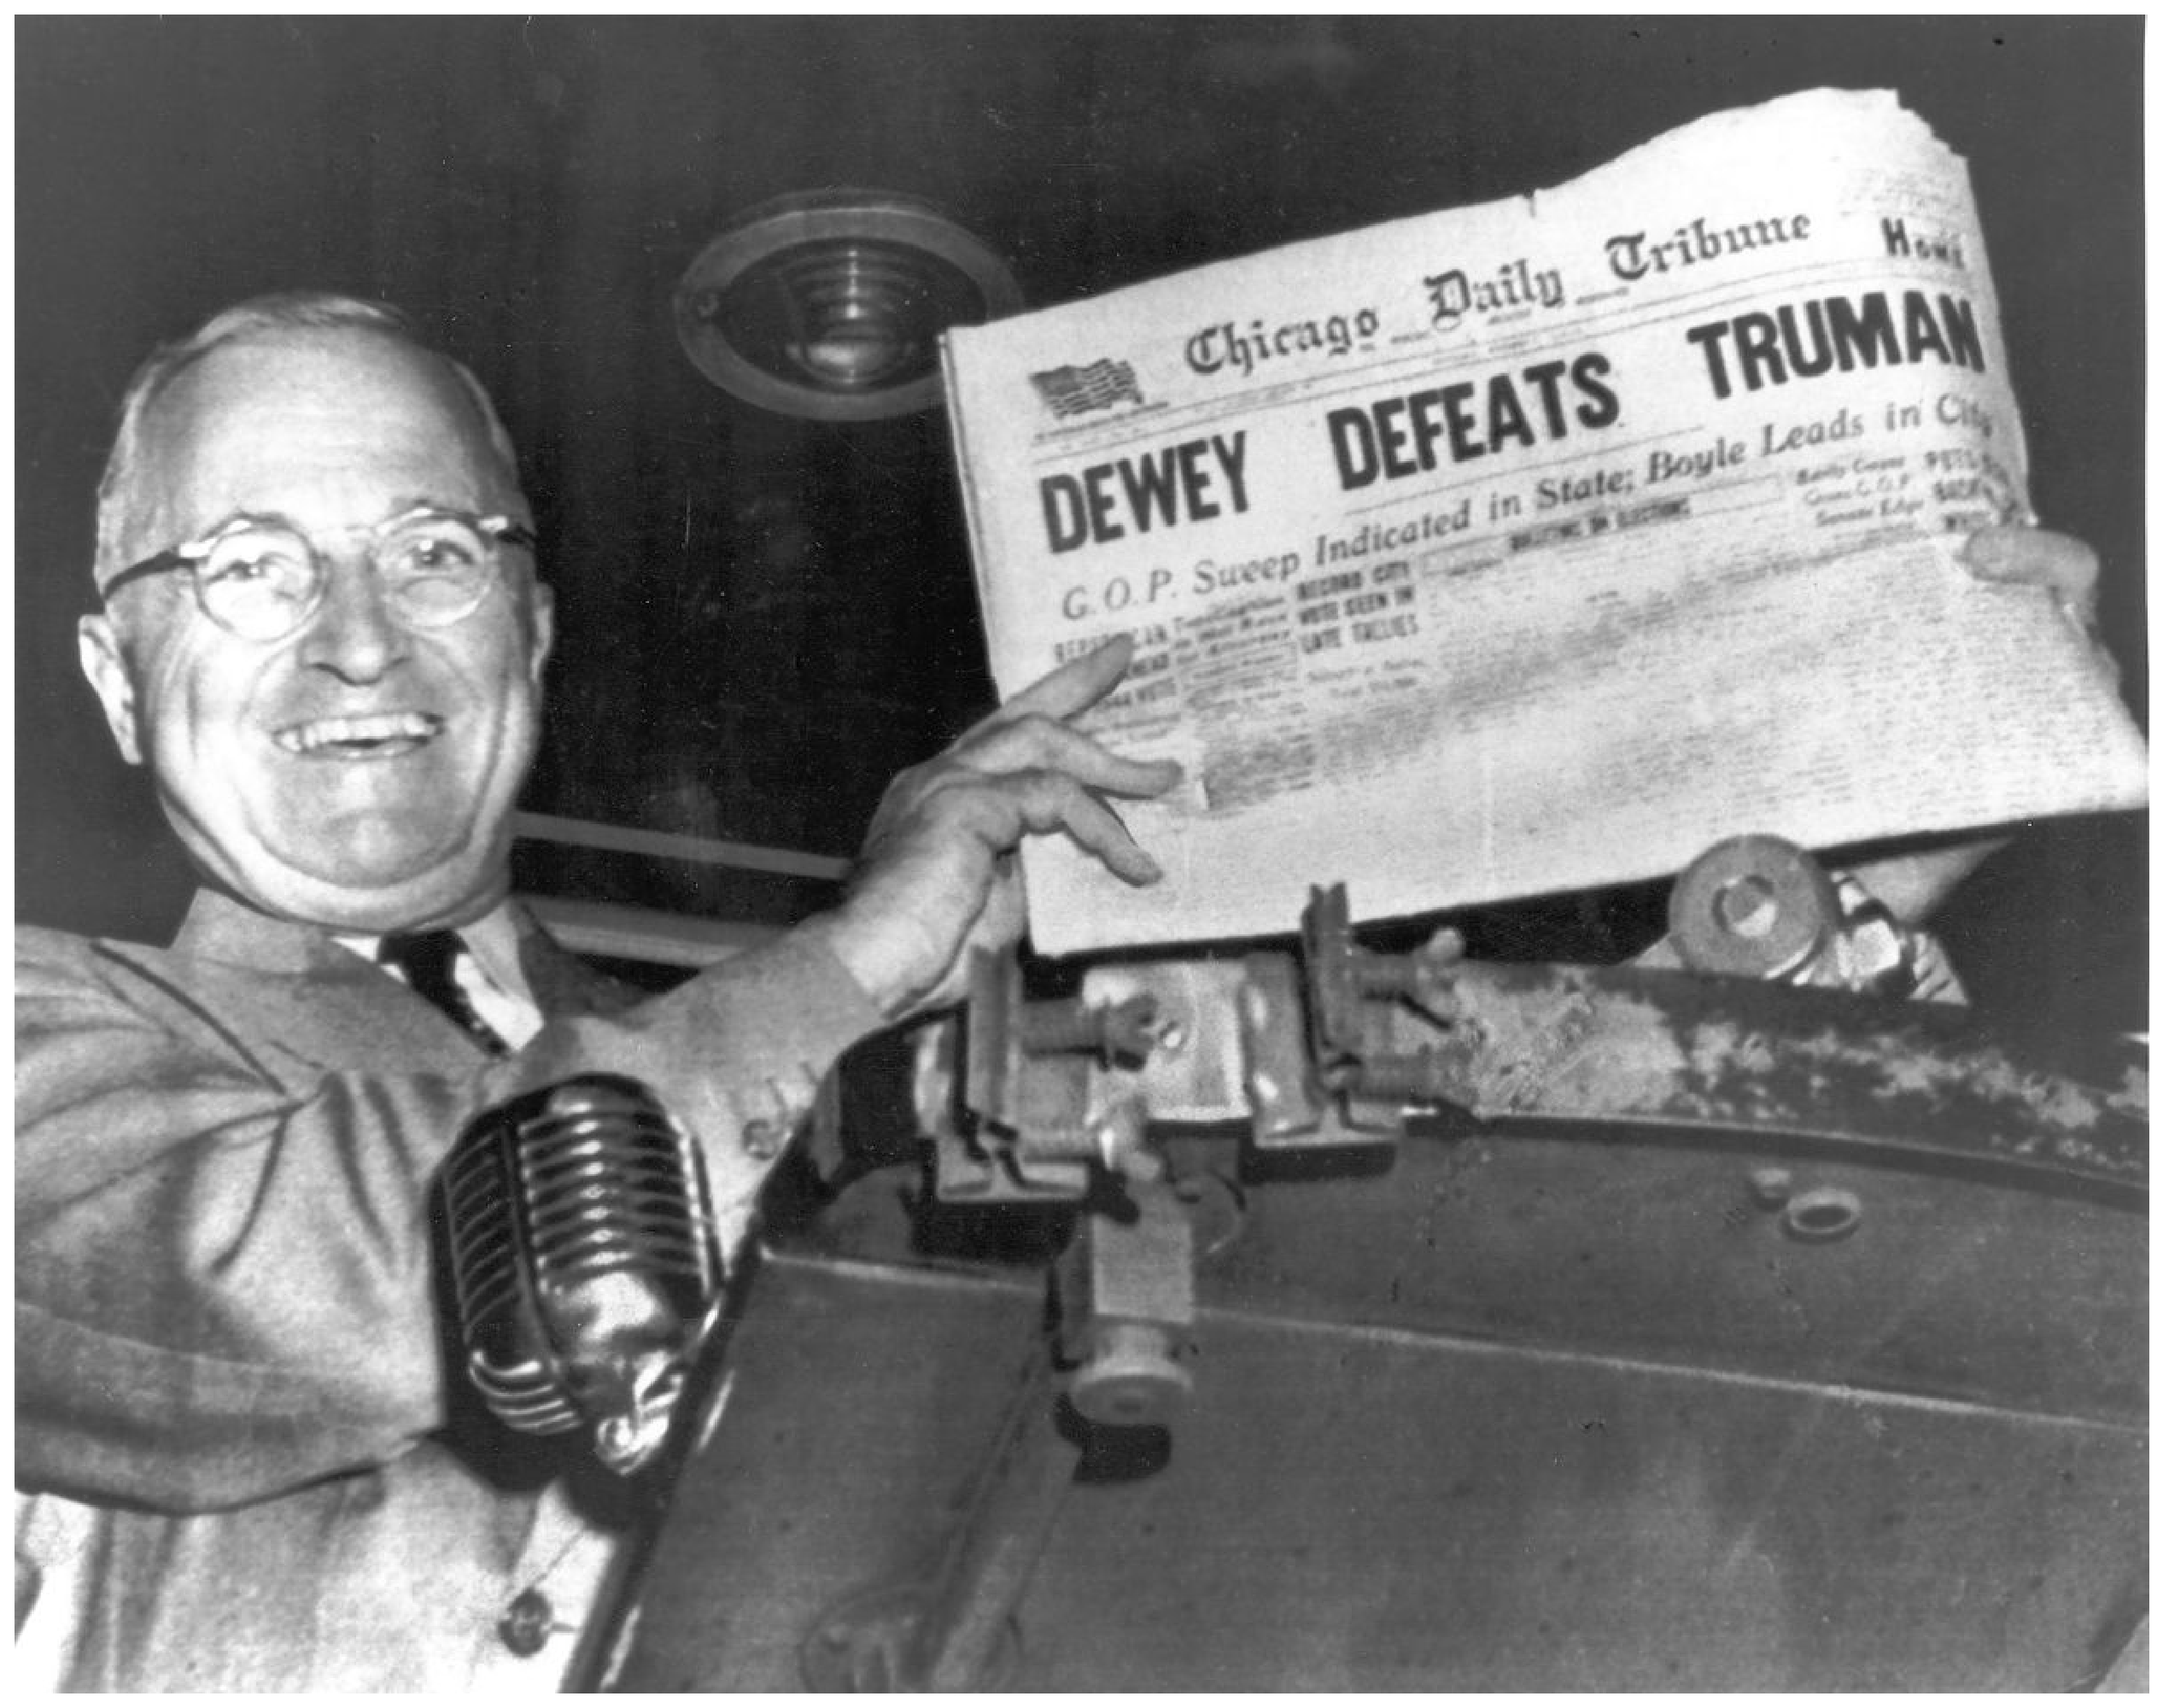
\includegraphics[height=1.5in]{Dewey.eps}\vspace{-10pt}
\end{center}

\footnotesize
\begin{itemize}
\item 1948 presidential election:  Harry Truman (Democratic incumbent who 
   ascended to the presidency when FDR died in office) ran agaist 
  Thomas Dewey (Republican district attourney from New York).
\item Three major polls predicted Dewey would win: Crossley (for the Hearst newspapers), Gallup and Roper (for \textit{Fortune} magazine)
\item Quota sampling (e.g., select specified numbers of people to poll by gender, race, age, etc.)
   did not accurately reflect the population.
\end{itemize}

\end{frame}

\subsection{Using Chance}
\begin{frame}
\frametitle{Using Chance}

\footnotesize
\begin{itemize}
\item Running a political poll is like sampling from a box of number tickets.
\item Simple random sampling:  
    \begin{itemize}
    \item \footnotesize Tickets drawn at random without replacement.
    \item \footnotesize  All tickets have equal likelihood of being chosen
    \end{itemize}
\item Multistage cluster sampling:
    \begin{itemize}
    \item \footnotesize Used to avoid challenges of randomly selected people being
          widely distributed across the country.
    \item \footnotesize Divide country into regions, regions into cities, etc.
    \item \footnotesize Randomly sample individuals from these specified areas.
    \item \footnotesize 
     Sample sizes are typically scaled to account for  relative populations of areas.
    \end{itemize}
\item \textit{The Islands}:  website for simulating samples from a fictional population:
\href{https://islands.smp.uq.edu.au}{https://islands.smp.uq.edu.au}
\item Probability methods are highly effective!  See Section 19.5.
\end{itemize}


\end{frame}

\subsection{Chance Error and Bias}
\begin{frame}
\frametitle{Chance Error and Bias}

\begin{itemize}
\item Running a political poll is like sampling from a box of number tickets.
\begin{center}
\scalebox{0.8}{\psframebox{253,785\;\psframebox{0}\,s\hspace{5pt}
     433,211\;\psframebox{1}\,s}}\vspace{5pt}
\end{center}

\item Bias:  sample does not represent the actual distribution of 0s and 1s in the box.
\item Chance error:
$\displaystyle
  \mbox{SE}_{\scriptsize\mbox{\%}} = \frac{\mbox{\footnotesize SD}_{\scriptsize\mbox{box}}}{\sqrt{n}}$
\end{itemize}
\label{lastpage}
\end{frame}


\end{document}


